\section{Experimental validation}
\label{sec:expe}

\subsection{Methodology}
\label{sec:exp-methodo}

This section briefly discusses our experimental setup for the evaluation of
\Moca.

All our experiment were run on  machines from Grid5000 \emph{Edel} cluster
\footnote{A full hardware description is available here
    \url{https://www.grid5000.fr/mediawiki/index.php/Grenoble:Hardware\#Edel}}.
    These machines are composed of $2$ quad core \texttt{Intel Xeon E5520}
    cadenced a $2.27GHz$ with
    $24 GB$ of RAM. Hyper threading was disabled during the experiment.

We deployed a \emph{Debian} \emph{Wheezy} environment running a Linux $3.X$
\DB{Linux version}.
\DB{Environment online ?}.
\DB{Results online ?}

We evaluate our tool on all the \NPB~\cite{Jin1999}. For
each benchmarks, we compare \Moca with the Pin~\cite{Luk05Pin} instrumentation
from Tabarnac~\cite{Beniamine15TABARNACRR}. This instrumentation traces every
memory accesses but record only the number of time each thread accesses to
each page, without any other information.

Each configuration of each plots was executed at least $30$ times. Each point
shows the arithmetic mean of all runs. The error bars represent
the standard error.

Except for the experiment on the influence of \Moca's parameters, on every
experiment, \Moca was run with it's default parameters. Which are a logging
process wakeup interval of $0.5s$ and a monitor thread wakeup interval
of $40ms$.


\subsection{Experiments}
\label{sec:expe-ovh}

\subsubsection{\Moca default parameters}

\begin{figure}[htb]
    \centering
    \begin{subfigure}{\linewidth}
        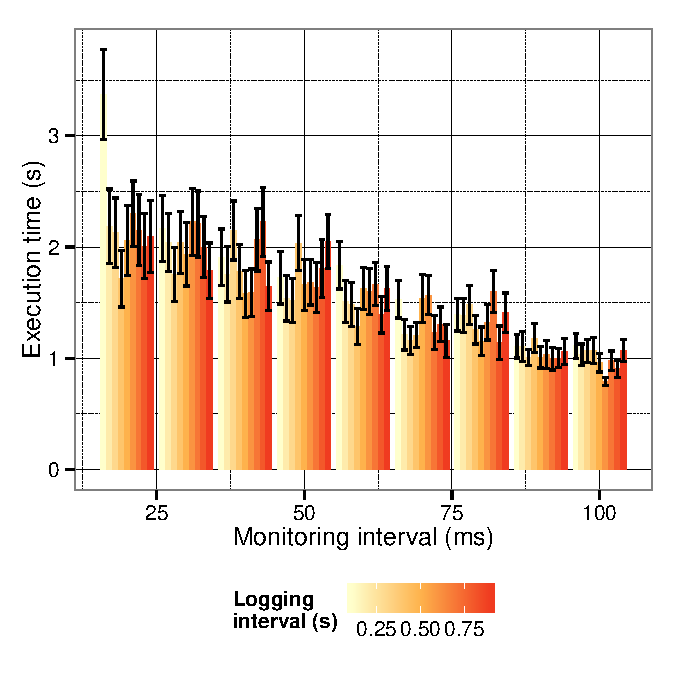
\includegraphics[width=\linewidth]{moca_param.pdf}
        \caption{Execution time.}
        \label{fig:param_time}
    \end{subfigure}

    \begin{subfigure}{\linewidth}
        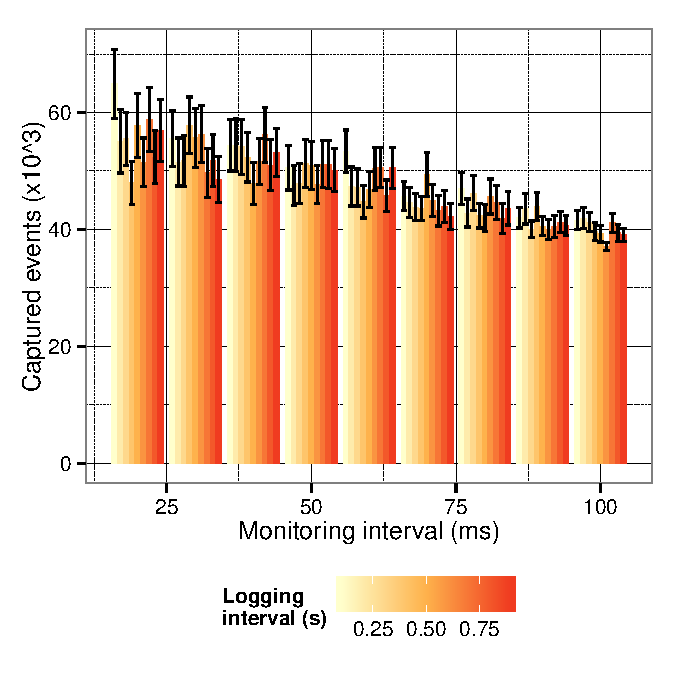
\includegraphics[width=\linewidth]{moca_param_events.pdf}
        \caption{Number of captured events.}
        \label{fig:param_evts}
    \end{subfigure}
    \caption{Influence of the wakeup intervals on \IS, class A.}
    \label{fig:param}
\end{figure}

Before comparing \Moca to existing tools, we need to evaluate the impact of
the wakeup intervals (logging daemon and monitor thread) on the trace
precision and on the overhead. To do so, we run the \IS benchmark under \Moca with
a wakeup interval from $0.1s$ to  $0.9s$ for the logging daemon and $20ms$ to
$100ms$. For each run, we measured \IS execution time and the number of
accesses captured. We choose \IS as it is on of the memory intensive \NPB

We can see in \fig{fig:param_time} that with a smaller wakeup interval for the
monitor thread than
$40ms$, performances are decreasing. Furthermore \fig{fig:param_evts} shows
that at this point he can capture a significant number of events. For this
value, waking up the logging process every $0.4s$ provides nice trade-off
between the execution time and the number of captured events.
\DB{$30$ runs here, let's do more to reduce the confidence intervals}

Using this knowledge, we set the default wakeup intervals to $40ms$ for the
monitor thread, and $0.4s$ for the logging thread.

\subsubsection{Comparison with existing tools}

Finally, to evaluate \Moca we needed a tool that also provide a superset of
the execution pages (see \ref{tab:tools-comp}) so we choose the Pin
instrumentation from Tabarnac. All the experiment presented here were run on
all the \NPB on class A.

\begin{figure}[htb]
    \centering
    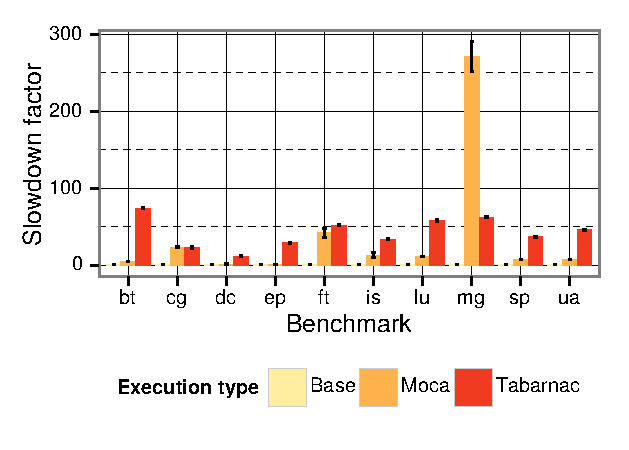
\includegraphics[width=\linewidth]{moca_overhead_nas.pdf}
    \caption{Slowdown of \Moca on the \NPB compared to
    Tabarnac.}
    \label{fig:ovh}
\end{figure}

\fig{fig:ovh} shows the slowdown of \Moca and Tabarnac compared to the
a normal execution of each benchmarks. We can identify three groups of
applications:  for \BT, \DC, \EP, \IS, \LU, \SP and \UA, \Moca is
significantly faster than Tabarnac. This set of benchmarks is interesting,
indeed if \EP is mostly doing parallel computation with only a few number of
memory accesses, \IS is memory intensive with a random memory access pattern
\BT, \LU and \SP are pseudo applications doing a significant usage of memory.
Finally \DC and \UA are categorised as \emph{unstructured computation,
parallel I/O and data movement} by the \NPB website
\footnote{\url{http://www.nas.nasa.gov/publications/npb.html}}. The second
group only contains memory oriented benchmarks (\CG and \FT). For this group
\Moca is as good as Tabarnac or a bit faster. Finally for \MG, \Moca seems to
be significantly slower than Tabarnac. Actually for this application, we
identified two behaviors: for $28$ runs out of $30$, the execution time under
\Moca was comparable to the on under Tabarnac, but for $2$ runs the execution
was $10$ time slower.
\DB{Actually 3 levels of runs for mg: 35sec, 120sec and 280sec \ldots}
This experiment shows that \Moca is significantly faster than existing tools
for most benchmarks, and at least as good for a few memory intensive
benchmarks.

\begin{figure}[htb]
    \centering
    \begin{subfigure}{\linewidth}
        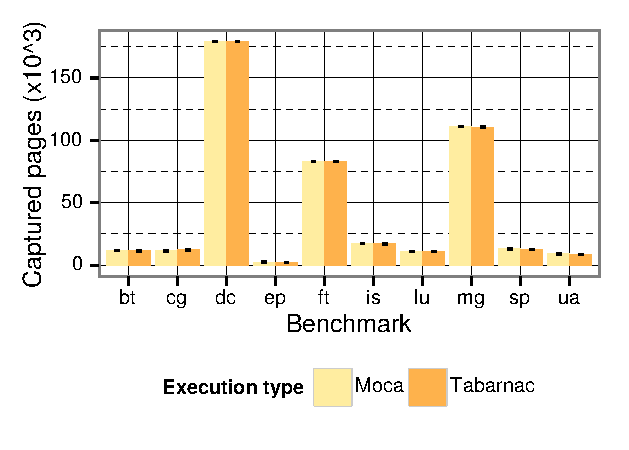
\includegraphics[width=\linewidth]{moca_pages_nas.pdf}
        \caption{Number of pages.}
        \label{fig:pages}
    \end{subfigure}
    \begin{subfigure}{\linewidth}
        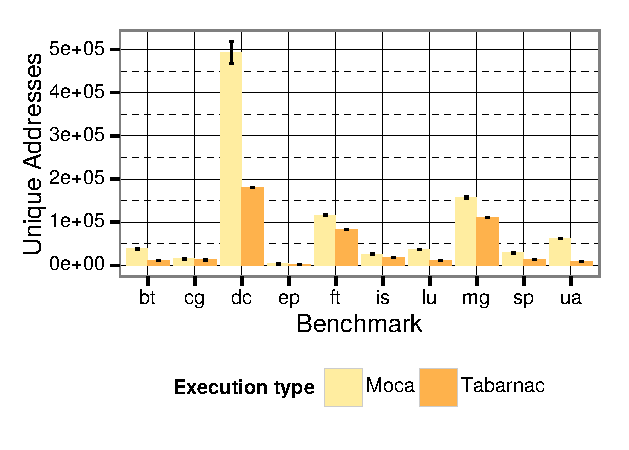
\includegraphics[width=\linewidth]{moca_addresses_nas.pdf}
        \caption{Number of unique addresses.}
        \label{fig:addr}
    \end{subfigure}
    \caption{Number of pages and unique addresses captured by \Moca and Tabarnac
    on the \NPB.}
    \label{fig:pages-addr}
\end{figure}

We then compared the number of pages and of unique addresses captured by \Moca
and Tabarnac during the previous experiment. As expected, we can see in
\fig{fig:pages} that both methods capture the exact same number of
pages which is the super set of all the accessed pages. Furthermore,
\fig{fig:addr} shows that \Moca also provides a more precise trace in
terms of unique addresses than Tabarnac. Indeed while \Moca provides a
superset of the pages of the execution, it store for each page fault the
actual address responsible for the page fault. Therefore it provide a trace
with the precision of the byte, while tools like Tabarnac needs to work at a
coarse granularity to limit their overhead.

\subsection{Summary}
\label{sec:expe-cncl}

We have tested \Moca under different application and with several parameters.
Our experiments, helped defining default parameters, and shows that with these
parameters, \Moca is at worst as slow as existing tools and in most of the
case faster. Moreover \Moca provides more precise traces than existing tools,
it is indeed the only tool able to provide a detailed trace with temporal,
spacial and sharing informations while providing guarantees on the information
loss during sampling.
